\chapter{Контрмера против атаки с навязыванием ключа} \label{ch:ch3}

%%%%%%%%%%%%%%%%%%%%%%%%%%%%%%%%%%%%%%%%%%%%%%%%%%%%%%%%%%%%%%%%%%%%%%%%%%%%%%%%%%%%%%%%%%%%%%%%%%%%%%%%%%%%%%%%%

\section{Атака с навязыванием ключа «поддельными» состояниями в системе квантовой коммуникации на боковых частотах} \label{ch:ch3/sec1}

В данной главе предлагается реализация атаки с <<поддельными>> состояниями на систему квантовой коммуникации на боковых частотах с используемым в приемном блоке детектором фотонов ID210. Как показали результаты исследования, изложенные во \ref{ch:ch2} главе, этот детектор подвержен выведению из режима Гейгера. Для осуществления успешной атаки между блоками легитимных отправителя и получателя располагается нелегитимный пользователь с аналогичным оборудованием. Всегда при рассмотрении возможностей злоумышленника предполагается, что они ограничены здравым смыслом и законами физики. Таким образом, принципиальная оптическая схема предлагаемой атаки представлена на рисунке \ref{fig:SCW_FSA}. 

 \begin{figure}[ht]
  \centering
  \includegraphics[scale=0.35]{scw-setup_FSA_rus1.pdf}
  \caption{Принципиальная оптическая схема предлагаемой атаки с <<поддельными состояниями>>}
  \label{fig:SCW_FSA}
\end{figure}

В состав подсистемы злоумышленника включена приёмная сторона, аналогичная получателю, и модифицированный под атаку блок отправителя. Первая часть подсистемы регистрирует срабатывания в соотвествии с протоколом. Применяемые квантовые состояния, которые привели к конструктивной интерференции, то есть за вычетом ошибок являются аналогичными по отношению к легитимному отправителю передаются в модифицированный блок отправителя. Модификация заключается в том, что в соотвествии с определёнными во \ref{ch:ch2} главе величинами, необходимыми для выведения детектора фотонов из режима Гейгера, источник формирует при помощи лазерного источника высокоинтенсивную несущую, затем в результате фазовой модуляции в спектре формируются боковые частоты, величина которых зависит от индекса модуляции. Весь спектр отправляется в приёмный блок, где в штатном режиме происходит повторная модуляция и интерференция сигналов на боковых частотах в зависимости от применяемых фазовых состояний. Затем отфильтровывается несущая частота, а боковые поступают на детектор одиночных фотонов. При этом мощность сигнала на боковых подбирается таким образом, чтобы её было достаточно для <<ослепления>> детектора и получения срабатывания в те моменты времени, когда злоумышленник отправляет известное, то есть совпавшее с легитимным отправителем, состояние. 


%%%%%%%%%%%%%%%%%%%%%%%%%%%%%%%%%%%%%%%%%%%%%%%%%%%%%%%%%%%%%%%%%%%%%%%%%%%%%%%%%%%%%%%%%%%%%%%%%%%%%%%%%%%%%%%%%
\section{Границы применимости атаки с навязыванием ключа} \label{ch:ch3/sec2}

Разберемся, чем обусловлены и ограничиваются параметры, которые модифицированная подсистема отправителя со стороны злоумышленника должна применять, чтобы успешно проводить предложенную атаку. 

В результате интерференции по аналогии со штатным режимом работы системы квантовой коммуникации с протоколом BB84 возможны 4 исхода, которые схематически представлены на рисунке \ref{fig:Palways}. Если разность фаз, применяемых при фазовой модуляции на стороне отправителя и получателя равна нулю, то интерференция конструктивна(КИ - <<конструктивная интерференция>>), то есть наблюдается усиление сигнала (при равных амплитудах  до четырехкратного увеличения). Если разность фаз равна $\pi$, то интерференция деструктивна (ДИ - <<деструктивная интерференция>>), то есть сигнал ослабляется до минимального уровня (шумов). Если используемые базисы не совпадают (НБ - <<несовпадение базисов>>), то разность фаз в обоих случаях равна $\pi/2$ и наблюдается половинный от максимального, соответствующего КИ, уровень мощности в классическом режиме, либо вероятность срабатывания 0,5 в квантовом режиме. 


 \begin{figure}[ht]
  \centering
  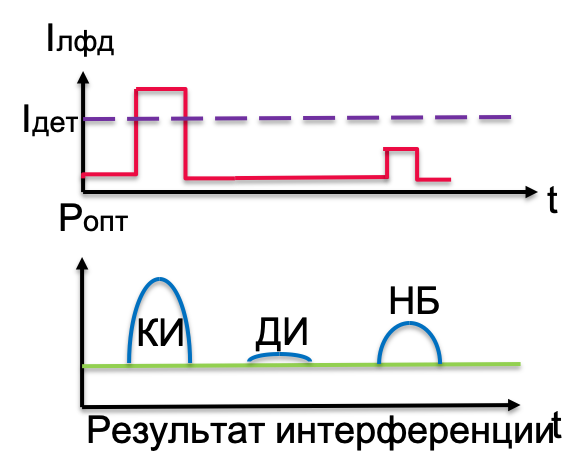
\includegraphics{Palways.png}
  \caption{Методика определения границ применимости}
  \label{fig:Palways}
\end{figure}


Стратегия злоумышленника максимально эффективна в том случае, когда легитимный пользователь с приёмником регистрирует срабатывания только в том случае, когда совпадение у отправителя и приёмной стороны злоумышленника было зафиксировано, а во все остальные моменты должно наблюдаться отсутствие срабатываний. Это условие будет автоматически выполняться в том случае, если фазовое состояние применяемое на приёмной стороне будет в противофазе с состоянием, пришедшим от модифицированной подсистемы злоумышленника, то есть будет наблюдаться ДИ. 

Однако, вариант с несовпадением базисов требует более внимательного рассмотрения. Для выполнения поставленного выше условия в случае несовпадения базисов требуется подобрать мощность контролирующих импульсов так, чтобы в результате интерференции порог срабатывания компаратора по току, протекающему в лавинном фотодиоде, не превысил уровень срабатывания, соответствущий току, необходимому для формирования импульса срабатывания. Это схематически представлено на рисунке \ref{fig:Palways}. \textit{Таким образом, накладывается ограничение сверху и снизу на оптическую мощность для контролирующих импульсов}. Чтобы приёмный блок не формировал срабатывания, не следует превышать величину оптической мощности $P_\text{никогда}$. А чтобы приёмный блок формировал состояния с единичной вероятностью, следует использовать мощность контролирующих оптических импульсов в пределах от $P_\text{никогда}$ до $P_\text{всегда\_предельное}$, которое равно удвоенному $P_\text{никогда}$:


\[
    \begin{cases}
     P < 2 \cdot P_\text{никогда} \\
     P \geqslant P_\text{всегда}
    \end{cases}
\]




Таким образом, детектор формирует импульс срабатывания только в случае совпадения используемых фазовых состояний, то есть конструктивной интерференции, и не должен формировать этот импульс при несовпадении базисов и деструктивной интерференции. Благодаря этому злоумышленник знает всю информацию о ключе, формируемом легитимными пользователями, а атака получила альтернативное название - <<навязывание ключа>>. Для разных оптических мощностей <<ослепления>> детектора фотонов определены границы применимости использования оптических мощностей контролирующих импульсов для формирования срабатывания и отсутствия срабатывания (рис. \ref{fig:Bounds}).  


 \begin{figure}[ht]
  \centering
  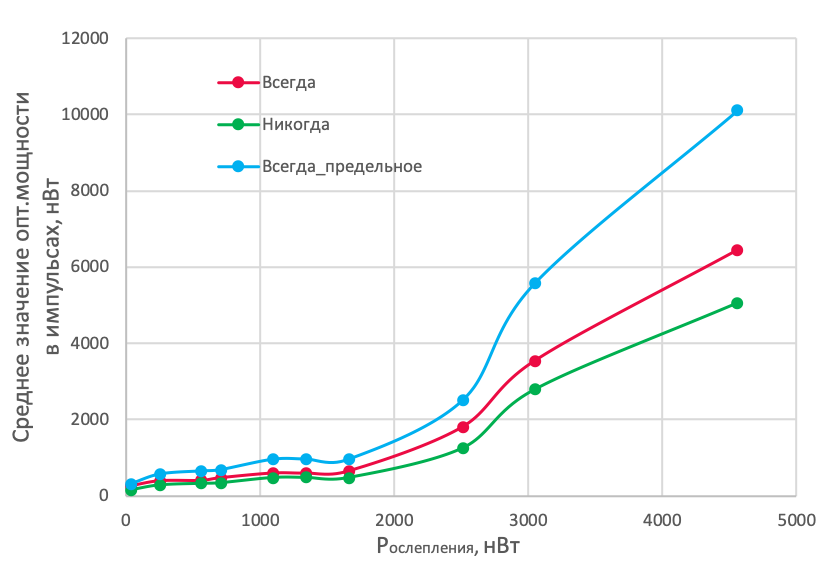
\includegraphics{Bounds.png}
  \caption{Границы применимости используемых оптических мощностей контролирующего импульса и засветки детектора}
  \label{fig:Bounds}
\end{figure}

%	\pagebreak

%%%%%%%%%%%%%%%%%%%%%%%%%%%%%%%%%%%%%%%%%%%%%%%%%%%%%%%%%%%%%%%%%%%%%%%%%%%%%%%%%%%%%%%%%%%%%%%%%%%%%%%%%%%%%%%%%
\section{Оценка возможностей злоумышленника при атаке с выведением детектора из режима Гейгера для систем квантовой коммуникации на боковых частотах} \label{ch:ch3/sec3}
 
 Приведем оценку необходимых параметров оптического излучения от модифицированной подсистемы злоумышленника для контроля детектора в приёмном блоке системы квантовой коммуникации на боковых частотах. Для этого воспользуемся полученными во \ref{ch:ch2} главе значениями. Известно, что блок получателя состоит из набора оптических компонентов (рис. \ref{fig:Bob}) со своими функциями и характеристиками, такими как вносимые потери и индекс модуляции.

 
 \begin{figure}[ht]
  \centering
  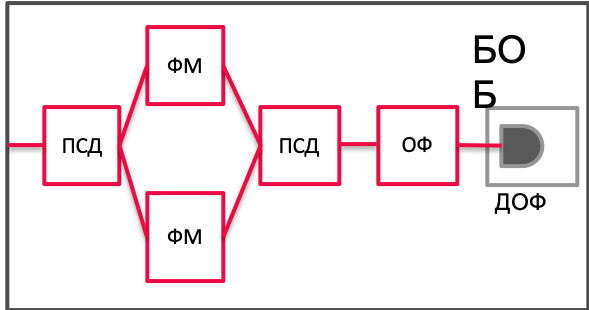
\includegraphics{Bob_scheme1.png}
  \caption{Принципиальная оптическая приемного модуля}
  \label{fig:Bob}
\end{figure}



Индекс модуляции, то есть соотношение энергии на центральной моде и на боковых равен 20:1. Таким образом, для того, чтобы детектор был ослеплен постоянной мощностью величиной в 35~нВт в спектре до фильтра должна быть величина в 20 раз больше.  Вносимые потери в блоке получателя составляют величину порядка 7 дБ. Расчеты представлены в таблице \ref{tab:blinding}.

 
 
\begin{table}
	\caption{\label{tab:blinding}Расчетные параметры для контроля детектора в системе квантовой коммуникации на боковых частотах.}
	\begin{tabular}[t]{c c c c}
	\hline\hline
	\makecell{Поддельное\\состояние\\злоумышленника\\мощность в...} & \makecell{Мощность для\\<<ослепления>> (нВт)} & $E_\text{всегда}$ (фДж) & $E_\text{никогда}$ (фДж) \\
	\hline
	\makecell{боковых после\\ фильтрации} & 35 & 25.8 & 15.4 \\
	\makecell{спектре перед\\ модуляцией} & 700 & 516 & 308 \\
	\makecell{спектре на входе\\ в приемный модуль} & 3056 & 2252 & 1345 \\
	\hline\hline
	\end{tabular}
\end{table}


\pagebreak

%%%%%%%%%%%%%%%%%%%%%%%%%%%%%%%%%%%%%%%%%%%%%%%%%%%%%%%%%%%%%%%%%%%%%%%%%%%%%%%%%%%%%%%%%%%%%%%%%%%%%%%%%%%%%%%%%

\section{Оптическая схема для противодействия атаке с <<ослеплением>> ДОФ} \label{ch:ch3/sec4}

В рамках данного исследования впервые в мире предлагается мера противодействия атакам с навязыванием ключа с использованием <<поддельных>> состояний с использованием преимуществ подхода к формированию квантовых состояний, а именно - вынесение квантового канала на боковые частоты фазомодулированного спектра.

Для определения попыток злоумышленника провести описанную выше атаку предлагается измерять интенсивность центральной оптической моды. Центральная мода отражается узкополосным фильтром на основе брэгговской решетки. Для того, чтобы её можно было измерить в схеме устанавливается волоконно-оптический циркулятор. Все излучение, которое после фазовых модуляторов в приемном блоке поступает на первый порт циркулятора направляется во второй порт на оптический фильтр. Отраженная центральная мода направляется в третий порт циркулятора. Для того, чтобы измерять центральную, которая, как показано в разделе \ref{ch:ch3/sec3}, должна быть порядка 700~нВт, предлагается использовать мониторный фотодиод. Так как предполагается, что у злоумышленника есть возможность подбирать интенсивность на центральной моде, то очевидным является то, что мониторный фотодиод, установленный на выходе с 3-го порта, можно также контролировать оптическими методами. Для того, чтобы избежать этого, предлагается использовать волоконно-оптическое зеркало, например широко доступное зеркало Фарадея, и пассивный оптический аттенюатор с фиксированной величиной вносимых потерь. Сам мониторный фотодиод предлагается устанавливать в 4-ом порту циркулятора. Таким образом, излучение с центральной модой поступает на 3-ий порт, проходит аттенюатор в прямом направлении, отражается от волоконного зеркала, проходит аттенюатор в обратном направлении и поступает на 4-й порт, где установлен мониторный фотодиод.         
 \begin{figure}[ht]
  \centering
  \includegraphics[scale=0.3]{scw-setup_Countermeasure.pdf}
  \caption{Принципиальная оптическая схема предлагаемой контрмеры против атаки с <<поддельными>> состояниями}
  \label{fig:countermeasure}
\end{figure}

\pagebreak

%%%%%%%%%%%%%%%%%%%%%%%%%%%%%%%%%%%%%%%%%%%%%%%%%%%%%%%%%%%%%%%%%%%%%%%%%%%%%%%%%%%%%%%%%%%%%%%%%%%%%%%%%%%%%%%%%
\section{Экспериментальная проверка контрмеры} \label{ch:ch3/sec5}

Для экспериментальной проверки предложенной контрмеры была собрана оптическая схема, воспроизводящая часть модифицированного подсистемы со стороны злоумышленника и блок получателя легитимного пользователя (рис. \ref{fig:Experimental_countermeasure}). 


 \begin{figure}[ht]
  \centering
  \includegraphics[scale=0.8]{Experimental_Countermeasure.pdf}
  \caption{Принципиальная оптическая схема предлагаемой контрмеры против атаки с <<поддельными>> состояниями}
  \label{fig:Experimental_countermeasure}
\end{figure}

Здесь стоит задача оценить работу в системе дополнительных элементов, введенных для активного мониторинга попыток злоумышленника вывести детектор одиночных фотонов и режима Гейгера постоянной оптической мощностью и контролировать срабатывания сильными оптическими импульсами. Для этих целей используются волоконно-оптический 4-ех портовый циркулятор, волоконное зеркало Фарадея и фиксированный аттенюатор розеточного типа с воздушным зазором на стыке феррул коннекторов зеркала и циркулятора. 

В модуле отправителя используются лазерный источник Л1, изолятор И, фазовый модулятор со встроенным поляризатором, подключенный электронике, программируемый оптический аттенюатор для регулировки выходной мощности с модуля. Управляющий сигнал представлен на рисунке \ref{fig:RF_sin_osc} и представляет из себя синус с частотой 4,8~ГГц. Амплитуда сигнала подбирается при помощи цифро-аналогового преобразователя ЦАП в пределах от 0 до 5~В таким образом, чтобы в результате модуляции 5~\% энергии несущей частоты распределялись на первой гармонике боковых частот.    


 \begin{figure}[ht]
  \centering
  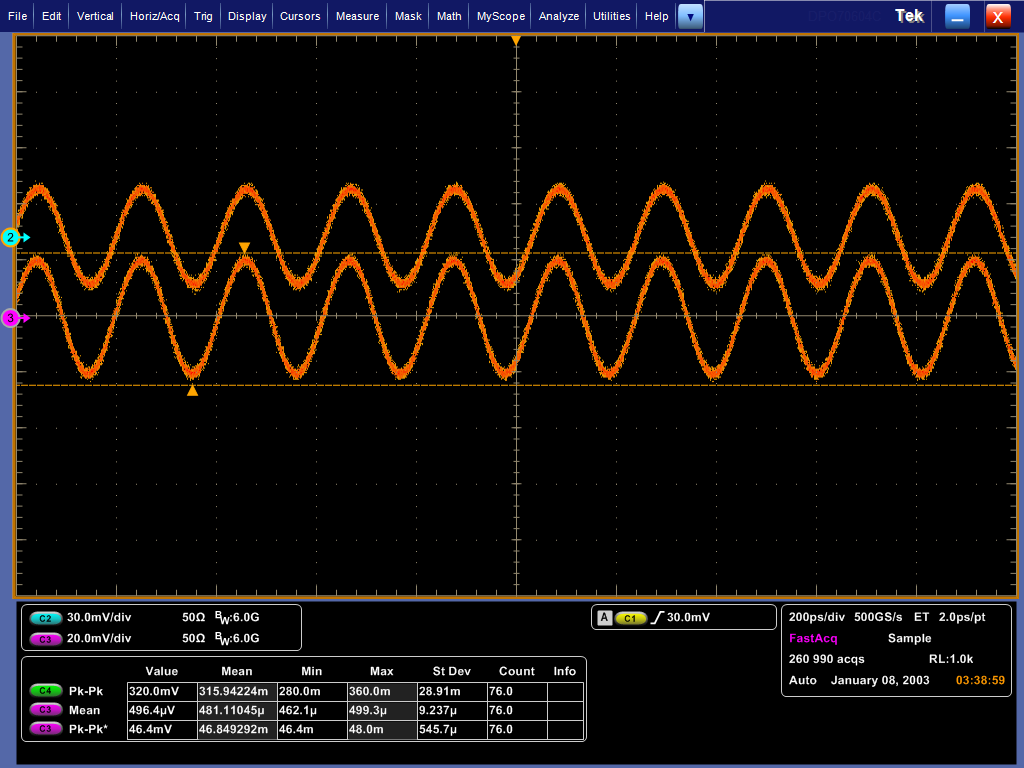
\includegraphics[scale=0.5]{sin_RF_mod_signal_constructive}
  \caption{Осциллограмма модулирующего сигнала в системе}
  \label{fig:RF_sin_osc}
\end{figure}


В приёмном модуле на 1-ый порт циркулятора Ц приходит излучение из модуля отправителя, которое с минимальными потерями не превышающими величину 1 дБ поступает на 2-ой порт с оптическим фильтром ОФ. Спектральная характеристика Л1 отстроена таким образом, чтобы центральная длина волны попадала в узкую полосу отражения ОФ, а боковые частоты проходили ОФ и поступали на детектор одиночных фотонов ДОФ. При мощности оптических импульсов на боковых частотах, достаточной для выведения ДОФ из режима счета фотонов в линейный, мощность на центральной частоте регистрировалась измерителем оптической мощности ФД2 FOD1204 с дипазоном 10 мВт - 50 пВт. В отсутствие в схеме аттенюатора зафиксированы следующие величины оптических мощностей (табл. \ref{tab:Circulator}). Таким образом, видно, что порядок величин, полученных экспериментально согласуется с расчетными из раздела \ref{ch:ch3/sec3} в отсутствие подсистемы модуляции в приёмном блоке. 


\begin{table}
	\caption{\label{tab:Circulator}Измеренные параметры при выведении детектора из режима счета фотонов в системе квантовой коммуникации.}
	\begin{tabular}[t]{c c c}
	\hline\hline
	\makecell{Мощность в...} & \makecell{Значение мощности (нВт)} & Значение мощности (дБм)  \\
	\hline
	\makecell{спектре на входе\\ в приемный модуль} & 2440 & -26.12 \\
	\makecell{боковых после\\ фильтрации} & 114.8 & -39.42 \\
	\makecell{отраженной от фильтра\\ центральной} & 1127 & -29.48  \\
	\makecell{на входе\\в мониторный диод} & 830 & -30.9  \\	
	\hline\hline
	\end{tabular}
\end{table}


\pagebreak
%%%%%%%%%%%%%%%%%%%%%%%%%%%%%%%%%%%%%%%%%%%%%%%%%%%%%%%%%%%%%%%%%%%%%%%%%%%%%%%%%%%%%%%%%%%%%%%%%%%%%%%%%%%%%%%%%
\section{Динамика оптической мощности на мониторном фотодиоде}\label{ch:ch3/sec6}

Благодаря граничным условиям на величину контролирующих оптических импульсов:

\[
    \begin{cases}
     P < 2 \cdot P_\text{никогда} \\
     P \geqslant P_\text{всегда}
    \end{cases}
\]

характеристикам устройств в приёмном блоке системы квантовой коммуникации, можно произвести количественную оценку требуемого диапазона чувствительности мониторного фотодиода и величину вносимого затухания аттенюатора, включенного в схему для защиты мониторного фотодиода от засветки злоумышленником. \textit{Для практических применений эта оценка является одним из весомых результатов исследования, так как позволяют достаточно простым способом с использованием преимуществ метода формирования квантовых состояний на боковых частотах отслеживать попытки злоумышленника по воздействию на детектор фотонов и навязыванию ключа легитимным пользователям}. 

На рисунке \ref{fig:Watchdog_photodiode} представлены две зависимости: нижний предел -- величина оптической мощности, которая требуется для выведения детектора фотонов из режима Гейгера и является минимальной необходимой для проведения успешной атаки злоумышленником; верхняя граница - величина оптической мощности, которая получена исходя из параметров приёмного модуля системы квантовой коммуникации и ограничения сверху на величину оптической мощности контролирующих импульсов. Минимальный уровень в соотвествии с расчетом составляет 0.7~мкВт, а максимальный - величину порядка 300~мкВт (в рамках данного исследования), однако на деле ограничен пороговой величиной ЛФД внутри ДОФ, при достижении которой ток становится слишком большим и диод сгорает, выводя из строя всё устройство. Типичной величиной являются единицы и десятки милливатт. 


С учётом данной зависимости можно оценить величину ослабления в фиксированном аттенюаторе, которой будет достаточно для защиты мониторного фотодиода от засветки, и при этом не потребуются дополнительные меры по расширению динамического диапазона чувствительности к входной оптической мощности в сторону увеличения, так как при оптических мощностях ниже единиц нановатт погрешность измерений становится достаточно высокой.   

Исходя из этого, величины аттенюации в 10~дБ достаточно, так как отраженная центральная на выходе с 3-го порта циркулятора прохоит через ослабляющий элемент в первый раз, а затем после отражения от зеркала во второй раз. Результирующее ослабление на 20~дБ, или в 100 раз, снизит минимальный уровень мощности на центральной частоте, которого достаточно для выведения детектора из режима счета фотонов, до величины порядка 7~нВт, что удовлетворяет требованиям, описанным выше. Максимальный уровень (в рамках данного исследования) снизится при этом примерно до 3~мкВт. 

 \begin{figure}[ht]
  \centering
  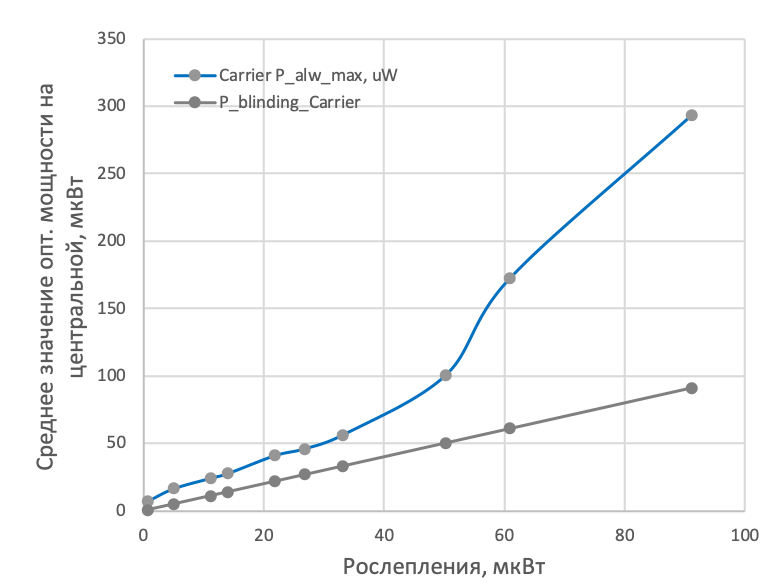
\includegraphics{images/Watchdog_photodiode.png}
  \caption{Динамика и границы оптической мощности на мониторном фотодиоде}
  \label{fig:Watchdog_photodiode}
\end{figure}


\pagebreak

%%%%%%%%%%%%%%%%%%%%%%%%%%%%%%%%%%%%%%%%%%%%%%%%%%%%%%%%%%%%%%%%%%%%%%%%%%%%%%%%%%%%%%%%%%%%%%%%%%%%%%%%%%%%%%%%%

\section{Учёт возможной контратаки со стороны злоумышленника}\label{ch:ch3/sec7}

Для оценки применимости предлагаемой идеи было проведено экспериментальное исследование контрмеры с добавлением в оптическую схему системы квантовой коммуникации на боковых частотах нескольких дополнительных компонентов (выделены красным цветом). В качестве мониторного фотодиода ФД использовался измеритель оптической мощности FOD 1204 (с диапазоном чувствительности фотоприёмника 10 мВт - 50 пВт). В качестве зеркала, отражающего центральную мощность обратно в циркулятор, использовалась волоконно-оптическое зеркало Фарадея (AC Photonics PMFRDMR13211). В качестве аттенюатора АТТ использовался фиксированный аттенюатор FC-FC типа розетка с воздушным зазором между поверхностями феррул волоконных коннекторов. Предлагаемая в данном исследовании контрмера, описанная выше \ref{ch:ch3/sec4}, основывается на том, что злоумышленник (Ева) формирует <<поддельные>> состояния (Faked-state attack) на тех же самых частотах оптического диапазона, что и модуль отправителя \ref{ch:ch3/sec1}. В таком случае, детектор переходит в линейный режим и становится подконтрольным злоумышленнику, начиная с некоторой величины постоянной оптической мощности. Затем, применяя контролирующие оптические импульсы с необходимой мощностью происходит навязывание злоумышленником срабатываний детектора. При этом ввиду особенности формирования квантовых состояний в системах на боковых частотах на приёмной стороне происходит спектральное разделение неинформативной несущей частоты и боковых частот, используемых для осуществления распределения ключа в качестве квантового сигнала. Боковые частоты попадают в спектр пропускания оптического фильтра, а несущая в спектр отражения, где осуществляется активный мониторинг её величины. Однако, полоса чувствительности детекторов фотонов на основе структур InGaAs/InP значительно шире (900-1700~нм). Таким образом, одним из вариантов контратаки злоумышленника с целью обойти предлагаемую контрмеру является изменение длины волны источника оптического излучения. Благодаря этому, в полосе отражения ОФ, и как следствие, на мониторном фотодиоде в приёмном модуле СКК сигнал будет отсутствовать, а <<контролирующие>> импульсы и оптические импульсы постоянного уровня оптической мощности для выведения ДОФ из режима счета фотонов позволят эффективно воздействовать на регистрирующее устройство блока получателя.

Решением является использование спектрально-селективного устройства на входе в блок получателя СКК, ограничивающего диапазон частот, поступающих в этот блок. Полоса пропускания должна быть достаточно узкой - не многим более величины 2 $\Omega$ (в нашем случае, 10~ГГц). В качестве такого устройства может быть использован волоконно-оптический фильтр на основе брэгговских решеток с термостабилизацией (такого же типа, как в ОФ в блоке получателя СКК). Однако, узкий диапазон частот характерен для работы в режиме отражения. Таким образом, в качестве спектрально-селективного устройства должна применяться связка волоконного оптического фильтра ОФ1 с волоконно-оптическим циркулятором. Вносимые потери фильтра и портов циркулятора составили 1.6 дБ. Преимуществом такого подхода является тот факт, что если злоумышленник будет отправлять импульсы непосредственно на частоте боковой, то в результате фазовой модуляции на ФМ2 в спектре появятся дополнительные компоненты, величина которых будет пропорциональная индексу модуляции (20:1), так что часть сигнала от злоумышленника, так или иначе будет попадать в полосу отражения ОФ2 и регистрироваться мониторным диодом).

Конечная схема контрмеры от атаки с поддельными состояниями для систем квантовой коммуникации на боковых частотах модулированного излучения с применением данной связки изображена на рисунке \ref{fig:scw-setup}. В результате экспериментального теста модифицированного приёмного блока системы квантовой коммуникации были получены следующие данные (\ref{tab:blinding2}). Расчетные величины (в 2 столбце) немного ниже полученных экспериментальным путем (5 столбец), ввиду флуктуаций параметров узлов системы, таких как экстинкция фильтра, вносимые потери. Выведение детектора из режима счета фотонов производилось с использованием описанной выше методики и полученных данных. На мониторном фотодиоде регистрировалась мощность в пределах чувствительности измерителя оптической мощности - 7,8~нВт. Таким образом, можно сформулировать требование к диапазону чувствительности мониторного диода - он не должен быть выше 1~нВт. Величина АТТ может быть подобрана с большей точностью для каждой конкретной системы квантовой коммуникации.

\begin{table}
	\centering \caption{\label{tab:blinding2}Параметры для осуществления контроля детектора ID210 в системе квантовой коммуникации на боковых частотах: расчетные (колонки 2-4) и полученные экспериментальным путем. Прочерки показывают нерелевантные данные (энергия несущей)}
	\begin{tabular}[t]{c c c c c}
	\hline\hline
	\makecell{<<Поддельные>>\\состояния в...} & \makecell{<<Ослепление>>\\ детектора (нВт)} & \makecell{$E_\text{всегда}$\\(фДж)} & \makecell{$E_\text{никогда}$\\(фДж)} & \makecell {Тестирование\\контрмеры (нВт)} \\
	\hline
	\makecell{Боковых частотах\\после фильтрации} & 35 & 25.8 & 15.4 & 114.8\\
	\makecell{Спектре перед\\ модуляцией} & 700 & 516 & 308 & 2440\\
	\makecell{Спектре на входе\\в получателя} & 4417 & 3256 & 1943 & 15395\\
	\makecell{Отраженная\\центральная частота} & 320 & -- & -- & 1127\\
	%\makecell{\edited{before}\\$10~\deci\bel$ ATT} & 310 & X & X & 830\\
	\makecell{Вход мониторного ФД} & 2.2 & -- & -- & 7.8\\
	\hline\hline
	\end{tabular}
\end{table}

\begin{figure}
	\centering \includegraphics{scw-setup.pdf}
	\caption{Система квантовой коммуникации на боковых частотах модулированного излучения. Устройства, окрашенные красным (серым в ч/б печати) цветом предлагаются в качестве контрмеры. Л - источник лазерного излучения; ФМ - фазовый модулятор; АТТ - аттенюатор; Ц- циркулятор; ОФ - оптический фильтр; ДОФ - детектор одиночных фотонов; ЗФ - зеркало Фарадея; ФД - мониторный фотодиод. Вставки показывают спектр сигнала в различных точках оптической схемы.}
	\label{fig:scw-setup}
\end{figure}

\pagebreak
%%%%%%%%%%%%%%%%%%%%%%%%%%%%%%%%%%%%%%%%%%%%%%%%%%%%%%%%%%%%%%%%%%%%%%%%%%%%%%%%%%%%%%%%%%%%%%%%%%%%%%%%%%%%%%%%%
\section{Выводы по главе} \label{ch:ch3/sec8}


В \ref{ch:ch3} главе показано, что измерение величины оптического излучения на несущей частоте, отраженного от оптического фильтра, при помощи мониторного фотодиода в приемном блоке системы квантовой коммуникации на боковых частотах в диапазоне от 7 нВт до 2,93 мкВт с применением дополнительных мер в виде пассивного оптического аттенюатора номиналом 10 дБ для его защиты позволяет противостоять атаке с выведением детектора одиночных фотонов из режима Гейгера и навязыванием ключа нелегитимным пользователем. Установлено требование по чувствительности мониторного фотодиода: необходимо, чтобы регистрировалась оптическая мощность от 1 нВт.
  